\onehalfspacing
\section{Đề số 9}
\graphicspath{{./img/}}
\begin{bt}
	\hfill
	\begin{enumerate}[1.]
		\item Tính giá trị các biểu thức sau:
		\begin{enumerate}[a.]
			\item $\mathrm{A}=\left(\frac{-3}{7}+\frac{4}{11}\right): \frac{7}{11}+\left(\frac{-4}{7}+\frac{7}{11}\right): \frac{7}{11}$
			\item $B=\frac{2^{12} \cdot 3^5-4^6 \cdot 9^2}{\left(2^2 \cdot 3\right)^6+8^4 \cdot 3^5}$
		\end{enumerate}
		\item Cho $\frac{x}{3}=\frac{y}{5}$. Tính giá trị biểu thức: $C=\frac{5 x^2+3 y^2}{10 x^2-3 y^2}$
	\end{enumerate}
	\loigiai{
		\begin{enumerate}[1.]
			\item \begin{enumerate}
				\item $
				A=\left(\frac{-3}{7}+\frac{4}{11}\right): \frac{7}{11}+\left(\frac{-4}{7}+\frac{7}{11}\right): \frac{7}{11}=\left(\frac{-3}{7}+\frac{4}{11}\right) \cdot \frac{11}{7}+\left(\frac{-4}{7}+\frac{7}{11}\right) \cdot \frac{11}{7} \\
				A=\frac{11}{7}\left[\left(\frac{-3}{7}+\frac{4}{11}\right)+\left(\frac{-4}{7}+\frac{7}{11}\right)\right]= \frac{11}{7}\left[\left(\frac{-3}{7}+\frac{-4}{7}\right)+\left(\frac{4}{11}+\frac{7}{11}\right)\right]\\=\frac{11}{7}[(-1)+1]=\frac{11}{7} \cdot 0=0
				$
				\item $
				\mathrm{B} =\frac{2^{12} \cdot 3^5-4^6 \cdot 9^2}{\left(2^2 \cdot 3\right)^6+8^4 \cdot 3^5}=\frac{2^{12} \cdot 3^5-\left(2^2\right)^6 \cdot\left(3^2\right)^2}{2^{12} \cdot 3^6+\left(2^3\right)^4 \cdot 3^5}\\=\frac{2^{12} \cdot 3^5-2^{12} \cdot 3^4}{2^{12} \cdot 3^6+2^{12} \cdot 3^5}=\frac{2^{12} \cdot 3^4(3-1)}{2^{12} \cdot 3^5(3+1)} \\
				\mathrm{B} =\frac{2^{12} \cdot 3^4 \cdot 2}{2^{12} \cdot 3^5 \cdot 4}=\frac{1}{6}$
			\end{enumerate}
			\item  Đặt $\frac{x}{3}=\frac{y}{5}=\mathrm{k} \Leftrightarrow\left\{\begin{array}{l}x=3 \mathrm{k} \\ \mathrm{y}=5 \mathrm{k}\end{array}\right.$. Khi đó:
			$$
			C=\frac{5 \mathrm{x}^2+3 \mathrm{y}^2}{10 \mathrm{x}^2-3 \mathrm{y}^2}=\frac{5(3 \mathrm{k})^2+3(5 \mathrm{k})^2}{10(3 \mathrm{k})^2-3(5 \mathrm{k})^2}=\frac{45 \mathrm{k}^2+75 \mathrm{k}^2}{90 \mathrm{k}^2-75 \mathrm{k}^2}=\frac{120 \mathrm{k}^2}{15 \mathrm{k}^2}=8
			$$
		\end{enumerate}
	} 
\end{bt}

\begin{bt}
	\hfill
	\begin{enumerate}[1.]
		\item Tìm các số $x, y, z$, biết:
		\begin{enumerate}[a.]
			\item $\frac{x}{2}=\frac{y}{3} ; \frac{y}{5}=\frac{z}{7}$ và $x+y+z=92$
			\item $(x-1)^{2018}+(2 y-1)^{2018}+|x+2 y-z|^{2019}=0$
		\end{enumerate}
		\item Tìm $x, y$ nguyên biết: $x y+3 x-y=6$
	\end{enumerate}
	\loigiai{
		\begin{enumerate}[1.]
			\item \begin{enumerate}
			\item Ta có: $\left\{\begin{array}{l}\frac{\mathrm{x}}{2}=\frac{\mathrm{y}}{3} \\ \frac{\mathrm{y}}{5}=\frac{\mathrm{z}}{7}\end{array} \Leftrightarrow\left\{\begin{array}{l}\frac{\mathrm{x}}{10}=\frac{\mathrm{y}}{15} \\ \frac{\mathrm{y}}{15}=\frac{\mathrm{z}}{21}\end{array} \Leftrightarrow \frac{\mathrm{x}}{10}=\frac{\mathrm{y}}{15}=\frac{\mathrm{z}}{21}\right.\right.$\\
			Áp dụng tính chất dãy tỉ số bằng nhau và $x+y+z=92$, ta được:\\
			$
		     \frac{x}{10}=\frac{y}{15}=\frac{z}{21}=\frac{x+y+z}{10+15+21}=\frac{92}{46}=2 \\
			\Rightarrow\left\{\begin{array}{l}
			\frac{x}{10}=2 \\
			\frac{y}{15}=2 \Leftrightarrow\left\{\begin{array}{l}
			x=20 \\
			y=30 \\
			z=42\\
			\end{array}\right. \\
			\frac{z}{21}=2
			\end{array}\right.
			$
			\item Ta có: \\
			$
				(\mathrm{x}-1)^{2016} \geq 0 \quad \forall \mathrm{x} \\
				(2 \mathrm{y}-1)^{2016} \geq 0 \quad \forall \mathrm{y} \\
				|\mathrm{x}+2 \mathrm{y}-\mathrm{z}|^{2017} \geq 0 \quad \forall \mathrm{x}, \mathrm{y}, \mathrm{z}\\
				 \Rightarrow(x-1)^{2016}+(2 y-1)^{2016}+|x+2 y-z|^{2017} \geq 0 \quad \forall x, y, z \\
				\text { Mà }(x-1)^{2016}+(2 y-1)^{2016}+|x+2 y-z|^{2017}=0\\
				\text { nên dấu "=" xảy ra } \Leftrightarrow\left\{\begin{array} { l } 
					{ ( \mathrm { x } - 1 ) ^ { 2 0 1 6 } = 0 } \\
					{ ( 2 \mathrm { y } - 1 ) ^ { 2 0 1 6 } = 0 } \\
					{ | \mathrm { x } + 2 \mathrm { y } - \mathrm { z } | ^ { 2 0 1 7 } = 0 }
					\end{array}\\
					 \Leftrightarrow \left\{\begin{array} { l } 
					{ \mathrm { x } = 1 } \\
					{ \mathrm { y } = \frac { 1 } { 2 } } \\
					{ 1 + 2 \cdot \frac { 1 } { 2 } - \mathrm { z } = 0 }
					\end{array}\\ 
					\Leftrightarrow \left\{\begin{array}{l}
					\mathrm{x}=1 \\
					\mathrm{y}=\frac{1}{2} \\
					\mathrm{z}=2
					\end{array}\right.\right.\right.
				$
		    \end{enumerate}
			\item Ta có: $x y+3 x-y=6 \Leftrightarrow x(y+3)-(y+3)=6-3$\\
			$
			\Leftrightarrow(x-1)(y+3)=3=1.3=3.1=(-1)(-3)=(-3)(-1)
			$\\
			Ta có bảng sau:\\
			$$\begin{array}{|c|c|c|c|c|}
				\hline \mathrm{x}-1 & 1 & 3 & -1 & -3 \\
				\hline \mathrm{y}+3 & 3 & 1 & -3 & -1 \\
				\hline \mathrm{x} & 2 & 4 & 0 & -2 \\
				\hline \mathrm{y} & 0 & -2 & -6 & -4 \\
				\hline
				\end{array}$$
				\text { Vậy: }(x ; y)=(2 ; 0)=(4 ;-2)=(0 ; 6)=(-2 ;-4)
	    \end{enumerate}
	} 
\end{bt}

\begin{bt}
	\hfill
	\begin{enumerate}[1.] 
		\item Tìm đa thức $\mathrm{A}$ biết: $A-\left(3 x y-4 y^2\right)=x^2-7 x y+8 y^2$
		\item Cho hàm số $y=f(x)=a x+2$ có đồ thị đi qua điểm $A\left(a-1 ; a^2+a\right)$.
		\begin{enumerate}[a.]
			\item Tìm a
			\item Với a vừa tìm được, tìm giá trị của $x$ thỏa mãn: $f(2 x-1)=f(1-2 x)$
		\end{enumerate}
	\end{enumerate}
	\loigiai{
		\begin{enumerate}[1.]
			\item Ta có: $A-\left(3 x y-4 y^2\right)=x^2-7 x y+8 y^2$\\
			$
			\begin{aligned}
			& A=x^2-7 x y+8 y^2+\left(3 x y-4 y^2\right) \\
			& A=x^2-4 x y+4 y^2
			\end{aligned}
			$
			\item \begin{enumerate}
				\item Vì đồ thị hàm số $\mathrm{y}=\mathrm{f}(\mathrm{x})=\mathrm{ax}+2$ đi qua điểm $\mathrm{A}\left(\mathrm{a}-1 ; \mathrm{a}^2+\mathrm{a}\right)$ nên: $a^2+a=a(a-1)+2 \Leftrightarrow a^2+a=a^2-a+2 \Leftrightarrow 2 a=2 \Leftrightarrow a=1$
				\item Với $a=1$ thì $y=f(x)=x+2$\\
				Ta có: $\mathrm{f}(2 \mathrm{x}-1)=\mathrm{f}(1-2 \mathrm{x}) \Leftrightarrow(2 \mathrm{x}-1)+2=(1-2 \mathrm{x})+2 \Leftrightarrow 4 \mathrm{x}=2 \Leftrightarrow \mathrm{x}=\frac{1}{2}$
			\end{enumerate}
		\end{enumerate}
	} 
\end{bt}

\begin{bt}
	Cho tam giác $A B C$ vuông tại $A$. Vẽ về phía ngoài tam giác $A B C$ các tam giác đều $A B D$ và $A C E$. Gọi $\mathrm{I}$ là giao điểm $B E$ và $C D$. Chứng minh rằng:
	\begin{enumerate}[a.]
		\item $B E=C D$
		\item $\triangle \mathrm{BDE}$ là tam giác cân
		\item $\mathrm{EIC}=60^{\circ}$ và IA là tia phân giác của DIE
	\end{enumerate}
	\loigiai{
		GT: $\triangle \mathrm{ABC}, \mathrm{A}=90^{\circ}, \Delta \mathrm{ABD}$ và $\triangle \mathrm{ACE}$ đều,
		$\mathrm{I}=\mathrm{BE} \cap \mathrm{CD}$\\ 
		KL:\\ 
		\begin{enumerate}
			\item  $\mathrm{BE}=\mathrm{CD}$
			\item $\triangle \mathrm{BDE}$ là tam giác cân
			\item $\mathrm{EIC}=60^{\circ}$ và $\mathrm{IA}$ là tia phân giác của DIE
		\end{enumerate}
		$$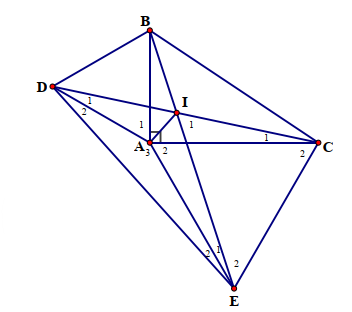
\includegraphics[width=0.55\textwidth]{9-4-lg.png}$$
		\begin{enumerate}
			\item $\text { Ta có: }\left\{\begin{array}{l}
				\mathrm{DAC}=\mathrm{A}_1+90^{\circ}=60^{\circ}+90^{\circ}=150^{\circ} \\
				\mathrm{BAE}=\mathrm{A}_2+90^{\circ}=60^{\circ}+90^{\circ}=150^{\circ}
				\end{array}\\ \Rightarrow \mathrm{DAC}=\mathrm{BAE}\right.$\\
				Xét $\triangle \mathrm{DAC}$ và $\triangle \mathrm{BAE}$ có:\\
                $
                \mathrm{DA} =\mathrm{BA}(\mathrm{GT}) \\
                \mathrm{DAC} =\mathrm{BAE}(\mathrm{CM} \text { trên) } \\
                \mathrm{AC} =\mathrm{AE}(\mathrm{GT}) \\
                \Rightarrow \Delta \mathrm{DAC} =\Delta \mathrm{BAE}(\mathrm{c}-\mathrm{g}-\mathrm{c}) \Rightarrow \mathrm{BE}=\mathrm{CD} \text { (Hai cạnh tương ứng) }
                $
				\item Ta có:  $\mathrm{A}_3+\mathrm{A}_1+\mathrm{BAC}+\mathrm{A}_2=360^{\circ}$\\
				$ \Leftrightarrow A_3+60^{\circ}+90^{\circ}+60^{\circ}=360^{\circ} \\
				 \Leftrightarrow A_3=150^{\circ} \\
				 \Rightarrow A_3=D A C=150^{\circ}$\\
				 Xét $\triangle \mathrm{DAE}$ và $\triangle \mathrm{BAE}$ có:\\
				 $
				 \mathrm{DA}=\mathrm{BA}(\mathrm{GT}) \\
				 \mathrm{A}_3=\mathrm{DAC}(\mathrm{CM} \text { trên })$\\
				 AE: Cạnh chung\\
				 $\Rightarrow \triangle \mathrm{DAE}=\triangle \mathrm{BAE}(\mathrm{c}-\mathrm{g}-\mathrm{c}) \\\Rightarrow \mathrm{DE}=\mathrm{BE}$ (Hai cạnh tương ứng)\\
				 $\Rightarrow \triangle B D E$ là tam giác cân tại $E$
				 \item Ta có: $\Delta \mathrm{DAC}=\Delta \mathrm{BAE}(\mathrm{CM}$ câu $\mathrm{a}) \Rightarrow \mathrm{E}_1=\mathrm{C}_1$ (Hai góc tương ứng)
				 Lại có: $\hat{\mathrm{I}}_1+\mathrm{E}_2+\mathrm{ICE}=180^{\circ}$ (Tổng 3 góc trong $\triangle \mathrm{ICE}$ )\\
				 $
				 \Leftrightarrow \hat{\mathrm{I}}_1+\left(\mathrm{AEC}-\mathrm{E}_1\right)+\left(\mathrm{C}_1+\mathrm{C}_2\right)=180^{\circ} \\
				 \Leftrightarrow \hat{\mathrm{I}}_1+60^{\circ}-\mathrm{E}_1+\mathrm{C}_1+60^{\circ}=180^{\circ} \\
				 \Leftrightarrow \hat{\mathrm{I}}_1+120^{\circ}=180^{\circ}\left(\text{Vì } \mathrm{E}_1=\mathrm{C}_1\right)$\\ 
				 $\Leftrightarrow \hat{\mathrm{I}}_1=60^{\circ}$\\
				 Vì $\triangle \mathrm{DAE}=\triangle \mathrm{BAE}\left(\mathrm{Cm}\right.$ câu b) $\Rightarrow \mathrm{E}_1=\mathrm{E}_2$ (Hai góc tương ứng)\\ $\Rightarrow \mathrm{EA}$ là tia phân giác của DEI (1)\\
				 $
				 \text{Vì }\left\{\begin{array}{l}
				 \triangle \mathrm{DAC}=\Delta \mathrm{BAE} \\
				 \triangle \mathrm{DAE}=\Delta \mathrm{BAE}
				 \end{array} \Rightarrow \triangle \mathrm{DAC}=\triangle \mathrm{DAE} \Rightarrow \mathrm{D}_1=\mathrm{D}_2 \text { (Hai góc tương ứng) }\\ \Rightarrow \mathrm{DA}\right. \text { là }
				 $
				 tia phân giác của EDC (2)\\
				 Từ (1) và (2) $\Rightarrow \mathrm{A}$ là giao điểm của 2 tia phân giác trong $\triangle \mathrm{DIE}\\ \Rightarrow \mathrm{IA}$ là đường phân giác thứ ba trong $\triangle$ DIE hay IA là tia phân giác của DIE
		\end{enumerate}
	}
\end{bt}

\begin{bt}
	\hfill
	\begin{enumerate}[1.] 
		\item Tìm số hữu tỉ $x$, sao cho tổng của số đó với nghịch đảo của nó có giá trị là một số nguyên.
		\item Cho các số a,b,c không âm thỏa mãn: $a+3 c=2016 ; a+2 b=2017$. Tìm giá trị lớn nhất của biểu thức $P=a+b+c$.
	\end{enumerate}
	\loigiai{
		\begin{enumerate}
			\item Gọi $x=\frac{m}{n}(m, n \in Z, n \neq 0,(m, n)=1)$. Khi đó:\\
			$
			\mathrm{x}+\frac{1}{\mathrm{x}}=\frac{\mathrm{m}}{\mathrm{n}}+\frac{\mathrm{n}}{\mathrm{m}}=\frac{\mathrm{m}^2+\mathrm{n}^2}{\mathrm{mn}}(1)
			$\\
			Để $x+\frac{1}{x}$ nguyên thì $\mathrm{m}^2+n^2: \mathrm{mn}$\\
			$
			\begin{gathered}
			\Rightarrow \mathrm{m}^2+\mathrm{n}^2 \vdots \mathrm{m} \\
			\Rightarrow \quad \mathrm{n}^2: \mathrm{m}\left(\text{vì } \mathrm{m^2} \vdots \mathrm{m}\right) \\
			\Rightarrow \quad \mathrm{n} \vdots \mathrm{m} \\
			\text { Mà }(\mathrm{m}, \mathrm{n})=1 \text { nên } \mathrm{m}=1 \text { hoặc } \mathrm{m}=-1
			\end{gathered}
			$
			\begin{enumerate}[*]
				\item Với m = 1:\\ 
				Từ (1), ta có: $\mathrm{x}+\frac{1}{\mathrm{x}}=\frac{1^2+\mathrm{n}^2}{1 \cdot \mathrm{n}}=\frac{1+\mathrm{n}^2}{\mathrm{n}}$. Để $\mathrm{x}+\frac{1}{\mathrm{x}}$ nguyên thì $1+\mathrm{n}^2 \vdots \mathrm{n} \Rightarrow 1 \vdots \mathrm{n}$ hay $\mathrm{n}= \pm$1
				\item Với m = -1:\\
				Từ (1), ta có: $\mathrm{x}+\frac{1}{\mathrm{x}}=\frac{(-1)^2+\mathrm{n}^2}{(-1) \cdot \mathrm{n}}=\frac{1+\mathrm{n}^2}{-\mathrm{n}}$. Để $\mathrm{x}+\frac{1}{\mathrm{x}}$ nguyên thì $1+\mathrm{n}^2:(-\mathrm{n}) \Rightarrow 1 \vdots(-\mathrm{n})$ hay $n= \pm 1$\\
                Khi đó $x=\frac{\mathrm{m}}{\mathrm{n}}=\frac{1}{1}=\frac{1}{-1}=\frac{-1}{1}=\frac{-1}{-1}$ hay $\mathrm{x}= \pm 1$
			\end{enumerate}
			\item Ta có: $\mathrm{a}+3 \mathrm{c}=2016$ (1) và $\mathrm{a}+2 \mathrm{~b}=2017$ (2)\\
			Từ (1) $\Rightarrow \mathrm{a}=2016-3 \mathrm{c}$\\
			Lấy (2) - (1) ta được: $2 \mathrm{~b}-3 \mathrm{c}=1 \Leftrightarrow \mathrm{b}=\frac{1+3 \mathrm{c}}{2}$.\\
			Khi đó:\\
			$
P=a+b+c=(2016-3 c)+\frac{1+3 c}{2}+c=\left(2016+\frac{1}{2}\right)+\frac{-6 c+3 c+2 c}{2}=2016 \frac{1}{2}-\frac{c}{2} .
$\\
Vì a, b, c không âm nên $P=2016 \frac{1}{2}-\frac{c}{2} \leq 2016 \frac{1}{2}, MaxP=2016 = \frac{1}{2}\\ \Leftrightarrow \mathrm{c}=0$
		\end{enumerate}
	}
\end{bt}